\documentclass{article}
\usepackage{graphicx, color}
\newcommand{\hlnumber}[1]{\textcolor[rgb]{0,0,0}{#1}}%
\newcommand{\hlfunctioncall}[1]{\textcolor[rgb]{.5,0,.33}{\textbf{#1}}}%
\newcommand{\hlstring}[1]{\textcolor[rgb]{.6,.6,1}{#1}}%
\newcommand{\hlkeyword}[1]{\textbf{#1}}%
\newcommand{\hlargument}[1]{\textcolor[rgb]{.69,.25,.02}{#1}}%
\newcommand{\hlcomment}[1]{\textcolor[rgb]{.18,.6,.34}{#1}}%
\newcommand{\hlroxygencomment}[1]{\textcolor[rgb]{.44,.48,.7}{#1}}%
\newcommand{\hlformalargs}[1]{\hlargument{#1}}%
\newcommand{\hleqformalargs}[1]{\hlargument{#1}}%
\newcommand{\hlassignement}[1]{\textbf{#1}}%
\newcommand{\hlpackage}[1]{\textcolor[rgb]{.59,.71,.145}{#1}}%
\newcommand{\hlslot}[1]{\textit{#1}}%
\newcommand{\hlsymbol}[1]{#1}%
\newcommand{\hlprompt}[1]{\textcolor[rgb]{.5,.5,.5}{#1}}%

\usepackage{color}%
 
\newsavebox{\hlnormalsizeboxclosebrace}%
\newsavebox{\hlnormalsizeboxopenbrace}%
\newsavebox{\hlnormalsizeboxbackslash}%
\newsavebox{\hlnormalsizeboxlessthan}%
\newsavebox{\hlnormalsizeboxgreaterthan}%
\newsavebox{\hlnormalsizeboxdollar}%
\newsavebox{\hlnormalsizeboxunderscore}%
\newsavebox{\hlnormalsizeboxand}%
\newsavebox{\hlnormalsizeboxhash}%
\newsavebox{\hlnormalsizeboxat}%
\newsavebox{\hlnormalsizeboxpercent}% 
\newsavebox{\hlnormalsizeboxhat}%
\newsavebox{\hlnormalsizeboxsinglequote}%
\newsavebox{\hlnormalsizeboxbacktick}%

\setbox\hlnormalsizeboxopenbrace=\hbox{\begin{normalsize}\verb.{.\end{normalsize}}%
\setbox\hlnormalsizeboxclosebrace=\hbox{\begin{normalsize}\verb.}.\end{normalsize}}%
\setbox\hlnormalsizeboxlessthan=\hbox{\begin{normalsize}\verb.<.\end{normalsize}}%
\setbox\hlnormalsizeboxdollar=\hbox{\begin{normalsize}\verb.$.\end{normalsize}}%
\setbox\hlnormalsizeboxunderscore=\hbox{\begin{normalsize}\verb._.\end{normalsize}}%
\setbox\hlnormalsizeboxand=\hbox{\begin{normalsize}\verb.&.\end{normalsize}}%
\setbox\hlnormalsizeboxhash=\hbox{\begin{normalsize}\verb.#.\end{normalsize}}%
\setbox\hlnormalsizeboxat=\hbox{\begin{normalsize}\verb.@.\end{normalsize}}%
\setbox\hlnormalsizeboxbackslash=\hbox{\begin{normalsize}\verb.\.\end{normalsize}}%
\setbox\hlnormalsizeboxgreaterthan=\hbox{\begin{normalsize}\verb.>.\end{normalsize}}%
\setbox\hlnormalsizeboxpercent=\hbox{\begin{normalsize}\verb.%.\end{normalsize}}%
\setbox\hlnormalsizeboxhat=\hbox{\begin{normalsize}\verb.^.\end{normalsize}}%
\setbox\hlnormalsizeboxsinglequote=\hbox{\begin{normalsize}\verb.'.\end{normalsize}}%
\setbox\hlnormalsizeboxbacktick=\hbox{\begin{normalsize}\verb.`.\end{normalsize}}%
\setbox\hlnormalsizeboxhat=\hbox{\begin{normalsize}\verb.^.\end{normalsize}}%



\newsavebox{\hltinyboxclosebrace}%
\newsavebox{\hltinyboxopenbrace}%
\newsavebox{\hltinyboxbackslash}%
\newsavebox{\hltinyboxlessthan}%
\newsavebox{\hltinyboxgreaterthan}%
\newsavebox{\hltinyboxdollar}%
\newsavebox{\hltinyboxunderscore}%
\newsavebox{\hltinyboxand}%
\newsavebox{\hltinyboxhash}%
\newsavebox{\hltinyboxat}%
\newsavebox{\hltinyboxpercent}% 
\newsavebox{\hltinyboxhat}%
\newsavebox{\hltinyboxsinglequote}%
\newsavebox{\hltinyboxbacktick}%

\setbox\hltinyboxopenbrace=\hbox{\begin{tiny}\verb.{.\end{tiny}}%
\setbox\hltinyboxclosebrace=\hbox{\begin{tiny}\verb.}.\end{tiny}}%
\setbox\hltinyboxlessthan=\hbox{\begin{tiny}\verb.<.\end{tiny}}%
\setbox\hltinyboxdollar=\hbox{\begin{tiny}\verb.$.\end{tiny}}%
\setbox\hltinyboxunderscore=\hbox{\begin{tiny}\verb._.\end{tiny}}%
\setbox\hltinyboxand=\hbox{\begin{tiny}\verb.&.\end{tiny}}%
\setbox\hltinyboxhash=\hbox{\begin{tiny}\verb.#.\end{tiny}}%
\setbox\hltinyboxat=\hbox{\begin{tiny}\verb.@.\end{tiny}}%
\setbox\hltinyboxbackslash=\hbox{\begin{tiny}\verb.\.\end{tiny}}%
\setbox\hltinyboxgreaterthan=\hbox{\begin{tiny}\verb.>.\end{tiny}}%
\setbox\hltinyboxpercent=\hbox{\begin{tiny}\verb.%.\end{tiny}}%
\setbox\hltinyboxhat=\hbox{\begin{tiny}\verb.^.\end{tiny}}%
\setbox\hltinyboxsinglequote=\hbox{\begin{tiny}\verb.'.\end{tiny}}%
\setbox\hltinyboxbacktick=\hbox{\begin{tiny}\verb.`.\end{tiny}}%
\setbox\hltinyboxhat=\hbox{\begin{tiny}\verb.^.\end{tiny}}%



\newsavebox{\hlscriptsizeboxclosebrace}%
\newsavebox{\hlscriptsizeboxopenbrace}%
\newsavebox{\hlscriptsizeboxbackslash}%
\newsavebox{\hlscriptsizeboxlessthan}%
\newsavebox{\hlscriptsizeboxgreaterthan}%
\newsavebox{\hlscriptsizeboxdollar}%
\newsavebox{\hlscriptsizeboxunderscore}%
\newsavebox{\hlscriptsizeboxand}%
\newsavebox{\hlscriptsizeboxhash}%
\newsavebox{\hlscriptsizeboxat}%
\newsavebox{\hlscriptsizeboxpercent}% 
\newsavebox{\hlscriptsizeboxhat}%
\newsavebox{\hlscriptsizeboxsinglequote}%
\newsavebox{\hlscriptsizeboxbacktick}%

\setbox\hlscriptsizeboxopenbrace=\hbox{\begin{scriptsize}\verb.{.\end{scriptsize}}%
\setbox\hlscriptsizeboxclosebrace=\hbox{\begin{scriptsize}\verb.}.\end{scriptsize}}%
\setbox\hlscriptsizeboxlessthan=\hbox{\begin{scriptsize}\verb.<.\end{scriptsize}}%
\setbox\hlscriptsizeboxdollar=\hbox{\begin{scriptsize}\verb.$.\end{scriptsize}}%
\setbox\hlscriptsizeboxunderscore=\hbox{\begin{scriptsize}\verb._.\end{scriptsize}}%
\setbox\hlscriptsizeboxand=\hbox{\begin{scriptsize}\verb.&.\end{scriptsize}}%
\setbox\hlscriptsizeboxhash=\hbox{\begin{scriptsize}\verb.#.\end{scriptsize}}%
\setbox\hlscriptsizeboxat=\hbox{\begin{scriptsize}\verb.@.\end{scriptsize}}%
\setbox\hlscriptsizeboxbackslash=\hbox{\begin{scriptsize}\verb.\.\end{scriptsize}}%
\setbox\hlscriptsizeboxgreaterthan=\hbox{\begin{scriptsize}\verb.>.\end{scriptsize}}%
\setbox\hlscriptsizeboxpercent=\hbox{\begin{scriptsize}\verb.%.\end{scriptsize}}%
\setbox\hlscriptsizeboxhat=\hbox{\begin{scriptsize}\verb.^.\end{scriptsize}}%
\setbox\hlscriptsizeboxsinglequote=\hbox{\begin{scriptsize}\verb.'.\end{scriptsize}}%
\setbox\hlscriptsizeboxbacktick=\hbox{\begin{scriptsize}\verb.`.\end{scriptsize}}%
\setbox\hlscriptsizeboxhat=\hbox{\begin{scriptsize}\verb.^.\end{scriptsize}}%



\newsavebox{\hlfootnotesizeboxclosebrace}%
\newsavebox{\hlfootnotesizeboxopenbrace}%
\newsavebox{\hlfootnotesizeboxbackslash}%
\newsavebox{\hlfootnotesizeboxlessthan}%
\newsavebox{\hlfootnotesizeboxgreaterthan}%
\newsavebox{\hlfootnotesizeboxdollar}%
\newsavebox{\hlfootnotesizeboxunderscore}%
\newsavebox{\hlfootnotesizeboxand}%
\newsavebox{\hlfootnotesizeboxhash}%
\newsavebox{\hlfootnotesizeboxat}%
\newsavebox{\hlfootnotesizeboxpercent}% 
\newsavebox{\hlfootnotesizeboxhat}%
\newsavebox{\hlfootnotesizeboxsinglequote}%
\newsavebox{\hlfootnotesizeboxbacktick}%

\setbox\hlfootnotesizeboxopenbrace=\hbox{\begin{footnotesize}\verb.{.\end{footnotesize}}%
\setbox\hlfootnotesizeboxclosebrace=\hbox{\begin{footnotesize}\verb.}.\end{footnotesize}}%
\setbox\hlfootnotesizeboxlessthan=\hbox{\begin{footnotesize}\verb.<.\end{footnotesize}}%
\setbox\hlfootnotesizeboxdollar=\hbox{\begin{footnotesize}\verb.$.\end{footnotesize}}%
\setbox\hlfootnotesizeboxunderscore=\hbox{\begin{footnotesize}\verb._.\end{footnotesize}}%
\setbox\hlfootnotesizeboxand=\hbox{\begin{footnotesize}\verb.&.\end{footnotesize}}%
\setbox\hlfootnotesizeboxhash=\hbox{\begin{footnotesize}\verb.#.\end{footnotesize}}%
\setbox\hlfootnotesizeboxat=\hbox{\begin{footnotesize}\verb.@.\end{footnotesize}}%
\setbox\hlfootnotesizeboxbackslash=\hbox{\begin{footnotesize}\verb.\.\end{footnotesize}}%
\setbox\hlfootnotesizeboxgreaterthan=\hbox{\begin{footnotesize}\verb.>.\end{footnotesize}}%
\setbox\hlfootnotesizeboxpercent=\hbox{\begin{footnotesize}\verb.%.\end{footnotesize}}%
\setbox\hlfootnotesizeboxhat=\hbox{\begin{footnotesize}\verb.^.\end{footnotesize}}%
\setbox\hlfootnotesizeboxsinglequote=\hbox{\begin{footnotesize}\verb.'.\end{footnotesize}}%
\setbox\hlfootnotesizeboxbacktick=\hbox{\begin{footnotesize}\verb.`.\end{footnotesize}}%
\setbox\hlfootnotesizeboxhat=\hbox{\begin{footnotesize}\verb.^.\end{footnotesize}}%



\newsavebox{\hlsmallboxclosebrace}%
\newsavebox{\hlsmallboxopenbrace}%
\newsavebox{\hlsmallboxbackslash}%
\newsavebox{\hlsmallboxlessthan}%
\newsavebox{\hlsmallboxgreaterthan}%
\newsavebox{\hlsmallboxdollar}%
\newsavebox{\hlsmallboxunderscore}%
\newsavebox{\hlsmallboxand}%
\newsavebox{\hlsmallboxhash}%
\newsavebox{\hlsmallboxat}%
\newsavebox{\hlsmallboxpercent}% 
\newsavebox{\hlsmallboxhat}%
\newsavebox{\hlsmallboxsinglequote}%
\newsavebox{\hlsmallboxbacktick}%

\setbox\hlsmallboxopenbrace=\hbox{\begin{small}\verb.{.\end{small}}%
\setbox\hlsmallboxclosebrace=\hbox{\begin{small}\verb.}.\end{small}}%
\setbox\hlsmallboxlessthan=\hbox{\begin{small}\verb.<.\end{small}}%
\setbox\hlsmallboxdollar=\hbox{\begin{small}\verb.$.\end{small}}%
\setbox\hlsmallboxunderscore=\hbox{\begin{small}\verb._.\end{small}}%
\setbox\hlsmallboxand=\hbox{\begin{small}\verb.&.\end{small}}%
\setbox\hlsmallboxhash=\hbox{\begin{small}\verb.#.\end{small}}%
\setbox\hlsmallboxat=\hbox{\begin{small}\verb.@.\end{small}}%
\setbox\hlsmallboxbackslash=\hbox{\begin{small}\verb.\.\end{small}}%
\setbox\hlsmallboxgreaterthan=\hbox{\begin{small}\verb.>.\end{small}}%
\setbox\hlsmallboxpercent=\hbox{\begin{small}\verb.%.\end{small}}%
\setbox\hlsmallboxhat=\hbox{\begin{small}\verb.^.\end{small}}%
\setbox\hlsmallboxsinglequote=\hbox{\begin{small}\verb.'.\end{small}}%
\setbox\hlsmallboxbacktick=\hbox{\begin{small}\verb.`.\end{small}}%
\setbox\hlsmallboxhat=\hbox{\begin{small}\verb.^.\end{small}}%



\newsavebox{\hllargeboxclosebrace}%
\newsavebox{\hllargeboxopenbrace}%
\newsavebox{\hllargeboxbackslash}%
\newsavebox{\hllargeboxlessthan}%
\newsavebox{\hllargeboxgreaterthan}%
\newsavebox{\hllargeboxdollar}%
\newsavebox{\hllargeboxunderscore}%
\newsavebox{\hllargeboxand}%
\newsavebox{\hllargeboxhash}%
\newsavebox{\hllargeboxat}%
\newsavebox{\hllargeboxpercent}% 
\newsavebox{\hllargeboxhat}%
\newsavebox{\hllargeboxsinglequote}%
\newsavebox{\hllargeboxbacktick}%

\setbox\hllargeboxopenbrace=\hbox{\begin{large}\verb.{.\end{large}}%
\setbox\hllargeboxclosebrace=\hbox{\begin{large}\verb.}.\end{large}}%
\setbox\hllargeboxlessthan=\hbox{\begin{large}\verb.<.\end{large}}%
\setbox\hllargeboxdollar=\hbox{\begin{large}\verb.$.\end{large}}%
\setbox\hllargeboxunderscore=\hbox{\begin{large}\verb._.\end{large}}%
\setbox\hllargeboxand=\hbox{\begin{large}\verb.&.\end{large}}%
\setbox\hllargeboxhash=\hbox{\begin{large}\verb.#.\end{large}}%
\setbox\hllargeboxat=\hbox{\begin{large}\verb.@.\end{large}}%
\setbox\hllargeboxbackslash=\hbox{\begin{large}\verb.\.\end{large}}%
\setbox\hllargeboxgreaterthan=\hbox{\begin{large}\verb.>.\end{large}}%
\setbox\hllargeboxpercent=\hbox{\begin{large}\verb.%.\end{large}}%
\setbox\hllargeboxhat=\hbox{\begin{large}\verb.^.\end{large}}%
\setbox\hllargeboxsinglequote=\hbox{\begin{large}\verb.'.\end{large}}%
\setbox\hllargeboxbacktick=\hbox{\begin{large}\verb.`.\end{large}}%
\setbox\hllargeboxhat=\hbox{\begin{large}\verb.^.\end{large}}%



\newsavebox{\hlLargeboxclosebrace}%
\newsavebox{\hlLargeboxopenbrace}%
\newsavebox{\hlLargeboxbackslash}%
\newsavebox{\hlLargeboxlessthan}%
\newsavebox{\hlLargeboxgreaterthan}%
\newsavebox{\hlLargeboxdollar}%
\newsavebox{\hlLargeboxunderscore}%
\newsavebox{\hlLargeboxand}%
\newsavebox{\hlLargeboxhash}%
\newsavebox{\hlLargeboxat}%
\newsavebox{\hlLargeboxpercent}% 
\newsavebox{\hlLargeboxhat}%
\newsavebox{\hlLargeboxsinglequote}%
\newsavebox{\hlLargeboxbacktick}%

\setbox\hlLargeboxopenbrace=\hbox{\begin{Large}\verb.{.\end{Large}}%
\setbox\hlLargeboxclosebrace=\hbox{\begin{Large}\verb.}.\end{Large}}%
\setbox\hlLargeboxlessthan=\hbox{\begin{Large}\verb.<.\end{Large}}%
\setbox\hlLargeboxdollar=\hbox{\begin{Large}\verb.$.\end{Large}}%
\setbox\hlLargeboxunderscore=\hbox{\begin{Large}\verb._.\end{Large}}%
\setbox\hlLargeboxand=\hbox{\begin{Large}\verb.&.\end{Large}}%
\setbox\hlLargeboxhash=\hbox{\begin{Large}\verb.#.\end{Large}}%
\setbox\hlLargeboxat=\hbox{\begin{Large}\verb.@.\end{Large}}%
\setbox\hlLargeboxbackslash=\hbox{\begin{Large}\verb.\.\end{Large}}%
\setbox\hlLargeboxgreaterthan=\hbox{\begin{Large}\verb.>.\end{Large}}%
\setbox\hlLargeboxpercent=\hbox{\begin{Large}\verb.%.\end{Large}}%
\setbox\hlLargeboxhat=\hbox{\begin{Large}\verb.^.\end{Large}}%
\setbox\hlLargeboxsinglequote=\hbox{\begin{Large}\verb.'.\end{Large}}%
\setbox\hlLargeboxbacktick=\hbox{\begin{Large}\verb.`.\end{Large}}%
\setbox\hlLargeboxhat=\hbox{\begin{Large}\verb.^.\end{Large}}%



\newsavebox{\hlLARGEboxclosebrace}%
\newsavebox{\hlLARGEboxopenbrace}%
\newsavebox{\hlLARGEboxbackslash}%
\newsavebox{\hlLARGEboxlessthan}%
\newsavebox{\hlLARGEboxgreaterthan}%
\newsavebox{\hlLARGEboxdollar}%
\newsavebox{\hlLARGEboxunderscore}%
\newsavebox{\hlLARGEboxand}%
\newsavebox{\hlLARGEboxhash}%
\newsavebox{\hlLARGEboxat}%
\newsavebox{\hlLARGEboxpercent}% 
\newsavebox{\hlLARGEboxhat}%
\newsavebox{\hlLARGEboxsinglequote}%
\newsavebox{\hlLARGEboxbacktick}%

\setbox\hlLARGEboxopenbrace=\hbox{\begin{LARGE}\verb.{.\end{LARGE}}%
\setbox\hlLARGEboxclosebrace=\hbox{\begin{LARGE}\verb.}.\end{LARGE}}%
\setbox\hlLARGEboxlessthan=\hbox{\begin{LARGE}\verb.<.\end{LARGE}}%
\setbox\hlLARGEboxdollar=\hbox{\begin{LARGE}\verb.$.\end{LARGE}}%
\setbox\hlLARGEboxunderscore=\hbox{\begin{LARGE}\verb._.\end{LARGE}}%
\setbox\hlLARGEboxand=\hbox{\begin{LARGE}\verb.&.\end{LARGE}}%
\setbox\hlLARGEboxhash=\hbox{\begin{LARGE}\verb.#.\end{LARGE}}%
\setbox\hlLARGEboxat=\hbox{\begin{LARGE}\verb.@.\end{LARGE}}%
\setbox\hlLARGEboxbackslash=\hbox{\begin{LARGE}\verb.\.\end{LARGE}}%
\setbox\hlLARGEboxgreaterthan=\hbox{\begin{LARGE}\verb.>.\end{LARGE}}%
\setbox\hlLARGEboxpercent=\hbox{\begin{LARGE}\verb.%.\end{LARGE}}%
\setbox\hlLARGEboxhat=\hbox{\begin{LARGE}\verb.^.\end{LARGE}}%
\setbox\hlLARGEboxsinglequote=\hbox{\begin{LARGE}\verb.'.\end{LARGE}}%
\setbox\hlLARGEboxbacktick=\hbox{\begin{LARGE}\verb.`.\end{LARGE}}%
\setbox\hlLARGEboxhat=\hbox{\begin{LARGE}\verb.^.\end{LARGE}}%



\newsavebox{\hlhugeboxclosebrace}%
\newsavebox{\hlhugeboxopenbrace}%
\newsavebox{\hlhugeboxbackslash}%
\newsavebox{\hlhugeboxlessthan}%
\newsavebox{\hlhugeboxgreaterthan}%
\newsavebox{\hlhugeboxdollar}%
\newsavebox{\hlhugeboxunderscore}%
\newsavebox{\hlhugeboxand}%
\newsavebox{\hlhugeboxhash}%
\newsavebox{\hlhugeboxat}%
\newsavebox{\hlhugeboxpercent}% 
\newsavebox{\hlhugeboxhat}%
\newsavebox{\hlhugeboxsinglequote}%
\newsavebox{\hlhugeboxbacktick}%

\setbox\hlhugeboxopenbrace=\hbox{\begin{huge}\verb.{.\end{huge}}%
\setbox\hlhugeboxclosebrace=\hbox{\begin{huge}\verb.}.\end{huge}}%
\setbox\hlhugeboxlessthan=\hbox{\begin{huge}\verb.<.\end{huge}}%
\setbox\hlhugeboxdollar=\hbox{\begin{huge}\verb.$.\end{huge}}%
\setbox\hlhugeboxunderscore=\hbox{\begin{huge}\verb._.\end{huge}}%
\setbox\hlhugeboxand=\hbox{\begin{huge}\verb.&.\end{huge}}%
\setbox\hlhugeboxhash=\hbox{\begin{huge}\verb.#.\end{huge}}%
\setbox\hlhugeboxat=\hbox{\begin{huge}\verb.@.\end{huge}}%
\setbox\hlhugeboxbackslash=\hbox{\begin{huge}\verb.\.\end{huge}}%
\setbox\hlhugeboxgreaterthan=\hbox{\begin{huge}\verb.>.\end{huge}}%
\setbox\hlhugeboxpercent=\hbox{\begin{huge}\verb.%.\end{huge}}%
\setbox\hlhugeboxhat=\hbox{\begin{huge}\verb.^.\end{huge}}%
\setbox\hlhugeboxsinglequote=\hbox{\begin{huge}\verb.'.\end{huge}}%
\setbox\hlhugeboxbacktick=\hbox{\begin{huge}\verb.`.\end{huge}}%
\setbox\hlhugeboxhat=\hbox{\begin{huge}\verb.^.\end{huge}}%



\newsavebox{\hlHugeboxclosebrace}%
\newsavebox{\hlHugeboxopenbrace}%
\newsavebox{\hlHugeboxbackslash}%
\newsavebox{\hlHugeboxlessthan}%
\newsavebox{\hlHugeboxgreaterthan}%
\newsavebox{\hlHugeboxdollar}%
\newsavebox{\hlHugeboxunderscore}%
\newsavebox{\hlHugeboxand}%
\newsavebox{\hlHugeboxhash}%
\newsavebox{\hlHugeboxat}%
\newsavebox{\hlHugeboxpercent}% 
\newsavebox{\hlHugeboxhat}%
\newsavebox{\hlHugeboxsinglequote}%
\newsavebox{\hlHugeboxbacktick}%

\setbox\hlHugeboxopenbrace=\hbox{\begin{Huge}\verb.{.\end{Huge}}%
\setbox\hlHugeboxclosebrace=\hbox{\begin{Huge}\verb.}.\end{Huge}}%
\setbox\hlHugeboxlessthan=\hbox{\begin{Huge}\verb.<.\end{Huge}}%
\setbox\hlHugeboxdollar=\hbox{\begin{Huge}\verb.$.\end{Huge}}%
\setbox\hlHugeboxunderscore=\hbox{\begin{Huge}\verb._.\end{Huge}}%
\setbox\hlHugeboxand=\hbox{\begin{Huge}\verb.&.\end{Huge}}%
\setbox\hlHugeboxhash=\hbox{\begin{Huge}\verb.#.\end{Huge}}%
\setbox\hlHugeboxat=\hbox{\begin{Huge}\verb.@.\end{Huge}}%
\setbox\hlHugeboxbackslash=\hbox{\begin{Huge}\verb.\.\end{Huge}}%
\setbox\hlHugeboxgreaterthan=\hbox{\begin{Huge}\verb.>.\end{Huge}}%
\setbox\hlHugeboxpercent=\hbox{\begin{Huge}\verb.%.\end{Huge}}%
\setbox\hlHugeboxhat=\hbox{\begin{Huge}\verb.^.\end{Huge}}%
\setbox\hlHugeboxsinglequote=\hbox{\begin{Huge}\verb.'.\end{Huge}}%
\setbox\hlHugeboxbacktick=\hbox{\begin{Huge}\verb.`.\end{Huge}}%
\setbox\hlHugeboxhat=\hbox{\begin{Huge}\verb.^.\end{Huge}}%
 

\def\urltilda{\kern -.15em\lower .7ex\hbox{\~{}}\kern .04em}%

\newcommand{\hlstd}[1]{\textcolor[rgb]{0,0,0}{#1}}%
\newcommand{\hlnum}[1]{\textcolor[rgb]{0.16,0.16,1}{#1}}
\newcommand{\hlesc}[1]{\textcolor[rgb]{1,0,1}{#1}}
\newcommand{\hlstr}[1]{\textcolor[rgb]{1,0,0}{#1}}
\newcommand{\hldstr}[1]{\textcolor[rgb]{0.51,0.51,0}{#1}}
\newcommand{\hlslc}[1]{\textcolor[rgb]{0.51,0.51,0.51}{\it{#1}}}
\newcommand{\hlcom}[1]{\textcolor[rgb]{0.51,0.51,0.51}{\it{#1}}}
\newcommand{\hldir}[1]{\textcolor[rgb]{0,0.51,0}{#1}}
\newcommand{\hlsym}[1]{\textcolor[rgb]{0,0,0}{#1}}
\newcommand{\hlline}[1]{\textcolor[rgb]{0.33,0.33,0.33}{#1}}
\newcommand{\hlkwa}[1]{\textcolor[rgb]{0,0,0}{\bf{#1}}}
\newcommand{\hlkwb}[1]{\textcolor[rgb]{0.51,0,0}{#1}}
\newcommand{\hlkwc}[1]{\textcolor[rgb]{0,0,0}{\bf{#1}}}
\newcommand{\hlkwd}[1]{\textcolor[rgb]{0,0,0.51}{#1}}

\definecolor{fgcolor}{rgb}{0,0,0}
\usepackage{framed}
\makeatletter
\newenvironment{kframe}{%
 \def\FrameCommand##1{\hskip\@totalleftmargin \hskip-\fboxsep
 \colorbox{shadecolor}{##1}\hskip-\fboxsep
     % There is no \@totalrightmargin, so:
     \hskip-\linewidth \hskip-\@totalleftmargin \hskip\columnwidth}%
 \MakeFramed {\advance\hsize-\width
   \@totalleftmargin\z@ \linewidth\hsize
   \@setminipage}}%
 {\par\unskip\endMakeFramed}
\makeatother

\definecolor{shadecolor}{rgb}{.97, .97, .97}
\newenvironment{knitrout}{}{} % an empty environment to be redefined in TeX

\newcommand{\SweaveOpts}[1]{}  % do not interfere with LaTeX
\newcommand{\SweaveInput}[1]{} % because they are not real TeX commands
\newcommand{\Sexpr}[1]{}       % will only be parsed by R

\usepackage{url, amsmath}

\title{{\tt SQM}: An R Package for Signature Quality Metrics\\The Utility Component}
\author{John A. Ramey}

\begin{document}




\maketitle

\section{Introduction}

The {\tt SQM} package contains the R code for the Signature Quality Metrics project
under the Signature Discovery Initiative (SDI) at the Pacific Northwest National
Laboratory (PNNL). The purpose of the SQM project is to provide subject-matter
experts (SMEs) with a set of tools to assess the quality of a set of signatures
in terms of accuracy, cost, and utility. For each of these components, we
have provided easy-to-use, accessible functions to measure the quality of
inputted signatures. In this document, we discuss the {\tt Utility} component
and demonstrate its usage with an example\footnote{Familarity with R
is recommended to fully comprehend our provided example.}.

The {\tt Utility} component of {\tt SQM} enables an SME to indicate his value
for a set of signature system attributes via a mathematical formulation. Paired
with other SQM components, such as {\tt Cost}, the {\tt Utility} component
equips an SME to identify signature systems that are of high valuee, are cost-effective,
and attain excellent accuracy.

In this document, we demonstrate the {\tt Utility} component of the {\tt SQM}
framework with a motivating example. We have completely fabricated the example
with contrived numbers and a fictitious SME, to illustrate a realistic
application of the {\tt SQM} framework.

\section{Example: Three Sensor Systems}

To motivate the {\tt Utility} component, we consider a hypothetical scnenario,
where we wish to compare three portable, human-carried sensor systems, which we
denote as:

\begin{itemize}
  \item Sensor {\tt A}
  \item Sensor {\tt B}
  \item Sensor {\tt C}.
\end{itemize}

Each of the three systems can be compared with a variety of metrics, such as
their accuracy in various, real-world scenarios and their cost. These two metrics
can be evaulated with the {\tt Accuracy} and {\tt Cost} components of the {\tt SQM}
package. Additionally, we may wish to compare the sensor systems in terms of their
overall usefulness, which may be difficult to compute, based on our subjective
evaluation of \emph{other attributes} of a sensor system. In this document, we
consider the following two \emph{other attributes} of the sensor systems:

\begin{enumerate}
  \item Weight, $w$
  \item Stand-off distance, $d$.
\end{enumerate}

For a deployed sensor system, the system's weight must be considered in addition to
its cost and accuracy. Consider, for example, a sensor that is highly accurate but
cannot be carried by a single human operator, due to its excessive weight. Clearly,
excessive weight is inhibiting and can reduce the sensor's practicality in the field.
So, we consider weight as an additional attribute with the understanding that lighter
is better.

Also, we consider the stand-off distance, which is the distance a sensor can be
from its target and maintain a specificied accuracy. The larger the stand-off
distance of a system is, the better. For illustration, we (naively?) assume that
the range of stand-off distances has little impact on the accuracy of detection.
That is, we assume that the accuracy of the sensor system practically does not
change within the considered range of stand-off distances. Moreover, we are not
interested in its impact on accuracy of detection. Rather, we wish to elicit from
the SME the perceived value of stand-off distance in terms of additional, perhaps
unknown, attributes corresponding to stand-off distance. For example, if a sensor
system were used at an airport security portal to detect illegal narcotics, we
may wish for the stand-off distance of the detection system to be large enough to
avoid alerting the miscreant that they are being detected; however, for this
example, a minimum recommended stand-off distance may not be clear, as it could
be subjective.

In our example problem, each of the two \emph{other attributes} will be used to
inform the SME of the three sensor systems' \emph{utility}. The purpose is to
formalize the subjectivity of the preference of the other attributes. For instance,
while we can easily say that \emph{heavy} sensors are impractical, we wish to be
upfront with what we mean by \emph{heavy} and also to combine our assessment of
weights with the stand-off distance.

To determine the SME's preference for the values of each attribute, we determine
a function that maps the observed values of the attribute to the unit interval.
Each attribute potentially can have its own utility (value) function if the
attributes can be assumed independent or separable. The elicitation of these
functions is non-trivial and can demand expertise from an expert in decision
analysis. In our example, we demonstrate an approach with simplicity in mind and
remark that realistic applications may require more sophisticated utility
functions.

Our goal is to provide a single utility score, measured in \emph{utils}, between
0 and 1, inclusively, that is used to rank each considered sensor system. The
sensor system with the maximum aggregated utility score is said to have the
highest value as defined by the elicited utility functions, which we discuss
below. Furthermore, the utility scores of each system can then be matched with
their respective accuracies, costs, and risks to identify the best overall
sensor.

\subsection{Utility Function Elicitation}

To illustrate the eliciation of the utility functions for each feature, 
we require some notation. Suppose that we have $n$ signatures, each with
$p$ attributes (features), that we wish to compare and determine the most
valuable signature. In our example, we have $n = 3$ signatures having $p = 2$
features. In this example, we make the simplifying assumption that \emph{weight}
and \emph{stand-off distance} are independent. We remark that this assumption
could be naive in realistic applications, but for demonstration of the {\tt SQM}
package, it allows us to effectively show the usage of the utility component.

We denote by $x_{ij}$ the $j$th observed feature for signature with
$i = 1, \ldots, n$ and $j = 1, \ldots, p$. Then, we write the utility function
for the $j$th feature $j$ as $U_j(x_{ij})$. Notice that the same utility function
is applied to each signature.

There are vast collections of functional forms that may be used for these utility
functions. As noted above, we are aiming for simplicity. First, we standardize
the value $x_{ij}$ to obtain a value in the unit interval. We use a reasonable
approach by asking the SME what range of values can the feature reasonably
expected to have. For example, although the weight of a system can possibly
be 2 million tons, this amount of weight is perhaps absurd to even consider
because no such system would ever be considered in practice. Thus, we ask that
the SME provide $x_j^{min}$ and $x_j^{max}$, the minimum and maximum reasonable
values for feature $j$, respectively. We standardize the $x_{ij}$ by

\begin{align*}
  x_{ij}^{*} = \frac{x_{ij} - x_j^{min}}{x_j^{max} - x_j^{min}},
\end{align*}
which is now between 0 and 1, inclusively.

For the $j$th feature, we write the utility function $U_{j}(x_{ij})$ as the
exponential function

\begin{align}
  U_{j}(x_{ij}) &= \frac{\exp\left\{-k \left(\dfrac{x_{ij} - x_j^{min}}{x_j^{max} - x_j^{min}}\right)\right\}}{\exp\{-k\} - 1}\nonumber\\
  &= \frac{\exp\{-k x_{ij}^{*}\} - 1}{\exp\{-k\} - 1}.\label{eq:exponential-utility}
\end{align}

The exponential function in \eqref{eq:exponential-utility} allows for a variety
of shapes that provide a reasonable valuation of the utility functions for our
example. The exponential rate of \eqref{eq:exponential-utility} is determined by
$k$. Also, notice that $U_j(x_j^{min}) = 0$ and $U_j(x_j^{max}) = 1$. After
the SE indicates the minimum and maximum acceptable values for the $j$th
feature, we need only determine the value of $k$. To elicit the value of $k$ from
the SME, we can ask for a single point that lies on the exponential curve. Rather
than bombarding the SME with equations to grok, we can implicitly determine the
value for $k$ through a straightforward exercise.

\subsubsection{Exercise to Determine the Shape of the Exponential Function}

Rather than asking the user for a shape parameter, we can ask the user for a
specified value of the $j$th feature and elicit a utility value through which
the exponential function in \eqref{eq:exponential-utility} must pass. As before,
we wish to avoid asking for functional values (much less, mentioning equations
at all). We instead can provide the user with the following scenario prompt:

\begin{quote}
  The purpose of this exercise is to rate the relative the desirability of
  different levels of a given attribute, assuming a fixed level of the other.

  The least desirable level is rated 0 out of 100 points, and the most desirable
  level a score of 100 out of 100 points. You will be given an intermediate level
  to which you should assign your personal rating between 0 and 100. Your rating
  should reflect how valuable it is to you to move from th eleast desirable to
  the intermediate level relative to moving from the least to the most desirable
  level.

  If it's not worth much to you to move from the least desirable to the
  intermediate level, then your rating should be relatively low (e.g. less than
  50 -- perhaps, much less than 50). Alternatively, if moving to the intermediate
  level is almost as valuable as moving all the way to the most desirable level,
  then your rating should be relatively high (e.g. more than 50).
\end{quote}

The functional form in \eqref{eq:exponential-utility} requires that the elicited
scores be scaled down to the unit interval. We can achieve this simply by
dividing the given scores by 100.

Next, we have the user provide a score for each feature with a well-crafted
question. For example, suppose that the SME has indicated that an acceptable
range of weights of a sensor system is between 0 and 60 pounds. The SME states
that values above 60 pounds can be excessive because the professional may already
be carrying a large amount of weight. We identify the midpoint of the values
to be 30 pounds. Then, we ask the SME the following question:

\begin{quote}
  On the scale from 0 to 100, how would you rate a signature system weighing 30
  pounds?
\end{quote}




Our fictitious SME responds with a score of 75, based on
the following reasoning. For systems that are light in weight, changes are hardly
noticeable to the professional and barely influence the perceived value. However,
for larger weights of deployed systems, small changes in weight are considerable
and severely influence the system's perceived value.

Next, we ask the SME a similar question to elicit a value function for stand-off
distance. The SME has indicated that an acceptable range of stand-off distances is
0 to 100 feet, so that the accuracy is near constant. As before, we compute the
midpoint to be 50 feet and ask:

\begin{quote}
  On the scale from 0 to 100, how would you rate a signature system with a
  stand-off distance of 50 feet?
\end{quote}




The SME provides the score of 30. The SME argues that
small stand-off distances only have a small amount of perceived value. For these
small distances, small changes in the distance have little influence on the
system's perceived value. Eventually though, for a system to achieve greater and
greater distances has huge implications for his project.

\subsection{Utility Aggregation via the Swing Weight Method}

Our goal is to aggregate the individual utility functions for each attribute to
summarize the overall utility of a specified signature system. More formally,
we wish to calculate the overall utility, $U_i$ for signature system,
$i = 1, \ldots, n$. For the signature system $i$, we wish to calculate the
utility of the $j$th attribute, $x_{ij}$ for each of the $p$ attributes
$(j = 1, \ldots, p)$. We write the overall utility $U_i$ for signature system
$i$ as

\begin{align}
  U_i = \sum_{j=1}^p \alpha_j U_j(x_{ij}),\label{eq:aggregate-utility}
\end{align}
with $\sum_{j=1}^p \alpha_j = 1$, where $\alpha_j$ weights the contribution of the $j$th
attribute to the overall utility. For our contrived example, we elicit the
weights, $\alpha_j$, from our fictition SME via the swing weights method.

We first asked our fictitious SME the following question: ``Suppose that we wish
to increase each \emph{other attribute} from its worst to best setting. Which
of the \emph{other attributes} is most imporant to shift from its worst-case to
its best-case scenario?'' The SME responded that a signature system simply cannot
be deployed if its stand-off distance is near zero because several scenario
contexts do not allow for a system to be close; for instance, if the signature
system is employed during a covert operation, then the operation's success may not
be possible if the system must be close to the target.

We then followed up our initial question with the following: ``Suppose that we
assigned a score of 100 on a scale of $0-100$ to shifting the stand-off distance
from its worst to best value. Relative to stand-off distance, on a scale from
$0-100$, what score would you assign a signature system's weight to shift it
from its worst possible value to its best possible value?''




The SME commented that although its largest (i.e. worst) weight is quite
impractical, it is conceivable that the system could still be deployed. However,
he noted that practically the system cannot be heavy. He then assigned a score
of 60 to weight.

To summarize, the SME assigned a score of 100 to
stand-off distance and a score of 60 to weight. We compute $\alpha_1$
for stand-off distance and $\alpha_2$ for weight by:

\begin{align*}
  \alpha_1 &= \frac{60}{100 + 60}
    = 0.375\\
  \alpha_2 &= \frac{100}{100 + 60}
    = 0.625
\end{align*}

\section{Implementation with the {\tt SQM} Package in {\tt R}}







In this section, we continue the above example and demonstrate how to employ the
Utility component of the {\tt SQM} framework's {\tt R} package to obtain results necessary
for determining a best sensor system. We require two sets of information from the
above example within the {\tt R} package:

\begin{enumerate}
  \item The elicited utility function values along with the swing weights
  \item The measured attributes for each sensor system
\end{enumerate}

The primary interface with the Utility component is through the {\tt afUtility} function, which
requires that the two sets of information be provided in separate CSV files. Before we discuss
the usage of the {\tt afUtility} function, we provide the formatting of the CSV files that will
be inputted.




First, we store the SME-elicited utility function arguments in the CSV file,  \textbf{utilityAttributes.csv}.
The column names should be provided, and the columns should be separated by commas. The CSV file has
the following form:

\begin{knitrout}
\definecolor{shadecolor}{rgb}{0.969, 0.969, 0.969}\color{fgcolor}\begin{kframe}
\begin{verbatim}
##   varNames x0   y0 xmin xmax weights increasing
## 1   weight 30 0.75    0   60   0.375      FALSE
## 2 standOff 50 0.30    0  100   0.625       TRUE
\end{verbatim}
\end{kframe}
\end{knitrout}


The values for {\tt x0} and {\tt y0} are the elicited midpoints and their corresponding scores, respectively, for
each attribute.

Next, we store the measured weights and stand-off distances for each sensor system (i.e. signature) in the CSV file,
\textbf{signatures.csv}.
The column names should be provided, and the columns should be separated by commas. The CSV file has
the following form:

\begin{knitrout}
\definecolor{shadecolor}{rgb}{0.969, 0.969, 0.969}\color{fgcolor}\begin{kframe}
\begin{verbatim}
##     signatureID weight standOff
## 1 sensorSystemA    100       20
## 2 sensorSystemB     25       50
## 3 sensorSystemC     40       80
\end{verbatim}
\end{kframe}
\end{knitrout}


Notice that the Sensor System A is the heaviest at 100 pounds, while Sensor System B is the lightest
at 25 pounds. Similarly, notice that Sensor System B has the farthest stand-off distance of
80. Our remaining question is: Which system is best? Clearly, Sensor System A is outperformed by
Sensor Systems B and C, but the cost and accuracy of this system might be worth the additional weight and reduced
stand-off distance. As we have discussed, the focus of this document is only on the Utility of the sensor systems.

Until now, we have yet to use the {\tt SQM} package directly. We are ready to do so here and illustrate the {\tt SQM}
package. Once the SME-elicited information has been properly formatted into CSV files, as above, we only have two
lines of code that we need to write. They are given here:
\begin{knitrout}
\definecolor{shadecolor}{rgb}{0.969, 0.969, 0.969}\color{fgcolor}\begin{kframe}
\begin{flushleft}
\ttfamily\noindent
\hlfunctioncall{library}\hlkeyword{(}\hlsymbol{SQM}\hlkeyword{)}\hspace*{\fill}\\
\hlstd{}\hlsymbol{utilityResults}{\ }\hlassignement{\usebox{\hlnormalsizeboxlessthan}-}{\ }\hlfunctioncall{afUtility}\hlkeyword{(}\hlargument{signaturesFile}{\ }\hlargument{=}{\ }\hlstring{"{}signatures.csv"{}}\hlkeyword{,}{\ }\hlargument{utilityAttributesFile}{\ }\hlargument{=}{\ }\hlstring{"{}utilityAttributes.csv"{}}\hlkeyword{,}\hspace*{\fill}\\
\hlstd{}{\ }{\ }{\ }{\ }\hlargument{outputFilePrefix}{\ }\hlargument{=}{\ }\hlstring{"{}utilityResults"{}}\hlkeyword{)}\mbox{}
\normalfont
\end{flushleft}
\end{kframe}
\end{knitrout}


The {\tt utilityResults} object contains useful information about the utility of each sensor
system along with its attributes. For instance, we can see the fitted utility function
information by attribute with

\begin{knitrout}
\definecolor{shadecolor}{rgb}{0.969, 0.969, 0.969}\color{fgcolor}\begin{kframe}
\begin{flushleft}
\ttfamily\noindent
\hlsymbol{utilityResults}\hlkeyword{\usebox{\hlnormalsizeboxdollar}}\hlsymbol{varUtilityFit}\mbox{}
\normalfont
\end{flushleft}
\begin{verbatim}
##               k xmin xmax increasing
## standOff -1.695    0  100       TRUE
## weight   -2.197    0   60      FALSE
\end{verbatim}
\end{kframe}
\end{knitrout}


To see graphs of the the elicted utility functions for each attribute, we need only call the {\tt plotUtility} function, which uses the information in {\tt varUtilityFit} above:

\begin{knitrout}
\definecolor{shadecolor}{rgb}{0.969, 0.969, 0.969}\color{fgcolor}\begin{kframe}
\begin{flushleft}
\ttfamily\noindent
\hlfunctioncall{plotUtility}\hlkeyword{(}\hlsymbol{utilityResults}\hlkeyword{)}\mbox{}
\normalfont
\end{flushleft}
\end{kframe}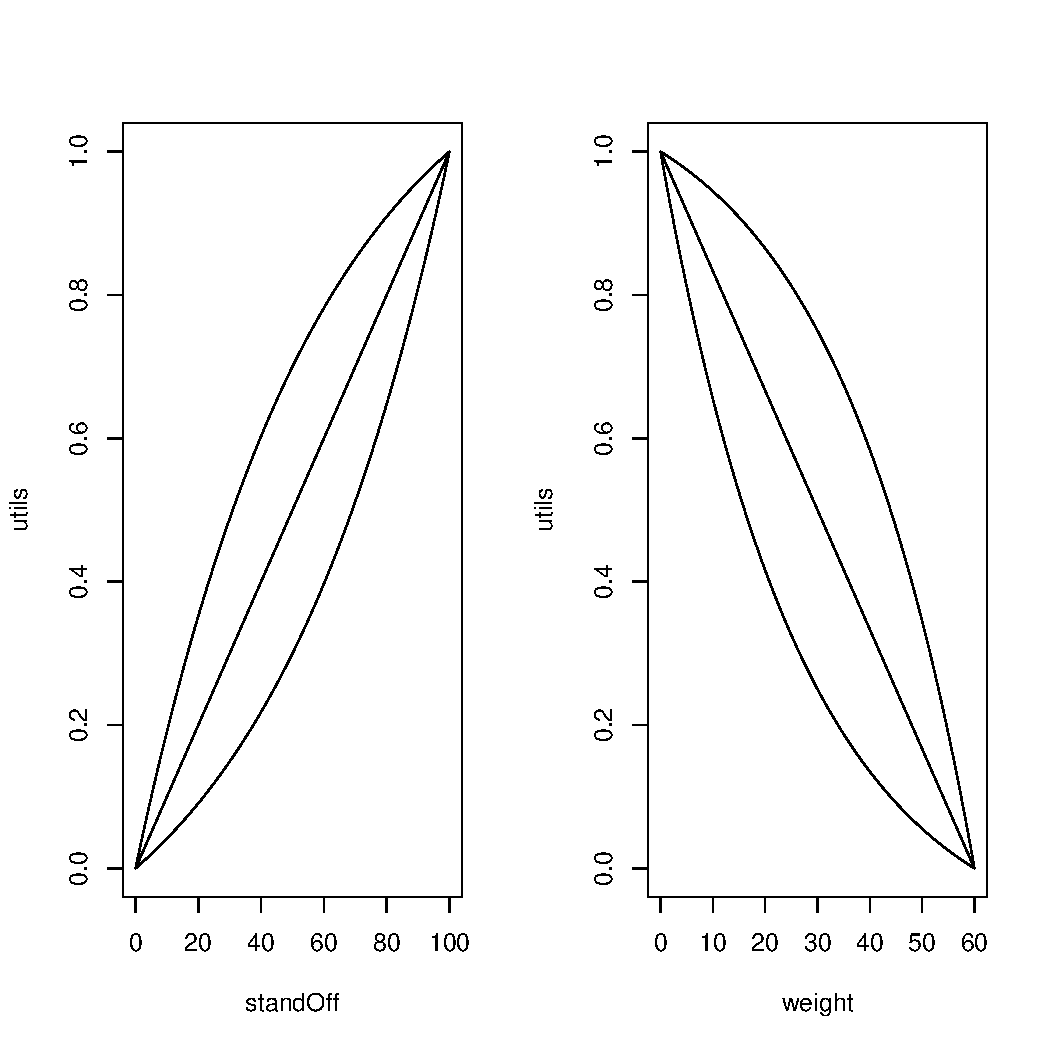
\includegraphics{plotUtility} 
\end{knitrout}


Finally, to see the aggregated utility scores for each attribute, we can look at the {\tt aggregate} object within the {\tt utilityResults} object:

\begin{knitrout}
\definecolor{shadecolor}{rgb}{0.969, 0.969, 0.969}\color{fgcolor}\begin{kframe}
\begin{flushleft}
\ttfamily\noindent
\hlsymbol{utilityResults}\hlkeyword{\usebox{\hlnormalsizeboxdollar}}\hlsymbol{aggregate}\mbox{}
\normalfont
\end{flushleft}
\begin{verbatim}
##     signatureID utility
## 1 sensorSystemA -2.3051
## 2 sensorSystemB  0.6205
## 3 sensorSystemC  0.6080
\end{verbatim}
\end{kframe}
\end{knitrout}


As we can see, using the elicited utility functions, Sensor Systems B and C are greatly superior
in terms of utility to Sensor System A. Sensor System B has a higher aggregated utility score than
Sensor System C, but the different might not be practically different.

\end{document}
